\documentclass[11pt]{article}

\usepackage[margin=1.1in]{geometry}
\usepackage[utf8]{inputenc}
\usepackage[T1]{fontenc}
\usepackage{lmodern}
\usepackage{microtype}
\usepackage{graphicx}
\usepackage{booktabs}
\usepackage{amsmath}
\usepackage[round]{natbib}
\usepackage[labelsep=period,font=small]{caption}
\usepackage{tikz}
\usetikzlibrary{positioning,arrows.meta}
\usepackage[hidelinks]{hyperref}
\usepackage{xcolor}

\newcommand{\repo}{\url{https://github.com/IshaanAyaan/slm-agents}}

\begin{document}

% ---------------------------------------------------------------- title page
\begin{titlepage}
  \centering
  \vspace*{3.2cm}
  {\LARGE\bfseries Specialized Small-Model Subagents\par}
  \vspace{0.6cm}
  {\Large Co-Designing a Fine-Tuned Small Language Model and a\\Task-Specific Harness for Cost-Efficient Multi-Agent Systems\par}
  \vspace{2.2cm}
  {\large Ishaan Ranjan \qquad Ganesh Talluri\par}
  \vspace{0.5cm}
  {\normalsize June 11, 2026\par}
  \vspace{2.2cm}
  \begin{minipage}{0.86\textwidth}
    \small
    All code, run logs, fine-tuning data and the statistics behind every number
    in this paper are public at \repo. The full experiment runs on one rented
    GPU in about ninety minutes for roughly five dollars and uses no paid API
    calls anywhere.
  \end{minipage}
  \vfill
\end{titlepage}

% ---------------------------------------------------------------- abstract
\begin{abstract}
\noindent
Multi-agent systems usually pair a strong orchestrator model with cheaper
worker models for delegated sub-tasks. The standard cost fix is to swap the
expensive worker for a small general-purpose model. We show that this swap
quietly fails and that a better option exists. We fine-tune a small model for
exactly one subagent role and pair it with a harness designed for that role,
where the harness owns state and memory while constraining and verifying every
action. A controlled two-by-three factorial design separates what the harness
contributes from what fine-tuning contributes and from what only their
combination produces. On a 200-task code-navigation benchmark built from five
held-out real repositories, judged against a strong 72B baseline that succeeds
95.5 percent of the time, our 3B specialist succeeds 94.5 percent of the time.
The difference is statistically indistinguishable (exact McNemar
$p = 0.82$) while cost per successful task falls by 84.8 percent
(bootstrap 95 percent CI [83.3, 86.1]). The naive swap is significantly worse
than the baseline on success and on cost at the same time. Each ingredient
alone makes things worse, and at 1.5B parameters the same fine-tuned model
scores 1.0 percent in the generic harness yet 93.5 percent in the co-designed
one. Specialization with co-design, not mere downsizing, is the cost-efficient
building block for multi-agent systems.
\end{abstract}

\vspace{0.5em}

% ---------------------------------------------------------------- 1
\section{Introduction}

The dominant pattern in agentic systems is hierarchical. A strong model
decomposes a task and hands sub-tasks to worker agents
\citep{yao2023react}. Workers are invoked far more often than the
orchestrator, so their cost dominates at scale, and the common response is to
replace the expensive frontier worker with a cheaper general-purpose model.

That replacement looks free on a per-token price sheet and is not free in
practice. The cheap general model still receives a broad system prompt and a
large tool list. It reasons in ways the narrow role never needed. Most
importantly it fails more, and failed attempts are not refunded. A failure
costs the worker's own tokens plus the orchestrator's tokens to detect the
problem and re-delegate. The honest unit of account is therefore
\emph{cost per successful task} rather than cost per token. Measured that
way, we find the naive swap can be strictly worse than the model it replaced.
In our headline experiment the swapped-in 3B model succeeded on 48.0 percent
of tasks against the 72B baseline's 95.5 percent, and its cost per successful
task was \emph{higher} than the baseline's, with a bootstrap confidence
interval that excludes parity.

We study a third option. Fine-tune a small model for exactly one recurring
subagent role, and run it inside a \emph{custom harness} built for that role.
The harness constrains the action space to the moves that are valid at the
current step. It compresses raw environment output into a minimal structured
observation. It keeps all durable state outside the model. It verifies every
action with cheap deterministic checks before the action counts, and when a
step fails it re-prompts only that step. The model is then fine-tuned, by
distilling verified trajectories from a large model
\citep{hinton2015distill, hsieh2023step}, to speak that harness's exact
input and output schema. The two artifacts are designed together, and the
central scientific claim of this paper is that they only work together.

Our contributions are the following.

\begin{enumerate}
  \item A method for co-designing a fine-tuned small language model with a
        task-specific harness, including a distillation pipeline that
        manufactures role-specific training data from verifier-clean large
        model trajectories.
  \item A controlled two-by-three factorial design that cleanly separates the
        harness effect from the fine-tuning effect and from their interaction,
        which addresses a confound that plagues comparisons of agent systems.
  \item Empirical results against a strong self-hosted 72B baseline over five
        held-out repositories and a 1.5B to 7B size sweep, with exact paired
        statistics, obtained for about five dollars of GPU time and zero API
        spend.
\end{enumerate}

% ---------------------------------------------------------------- 2
\section{Background and related work}

Three observations motivate the design. First, scaffolding matters as much as
weights. Holding a model fixed and changing only its agent scaffold moves
benchmark scores by large margins, which is well documented in the agent
literature around tool use and acting-while-reasoning patterns
\citep{yao2023react} and in software-engineering benchmarks where harness
details dominate outcomes \citep{jimenez2024swebench}. Second, small models
fine-tuned for narrow tasks can match much larger general models on those
tasks at a fraction of the serving cost, and distillation is the standard
mechanism for transferring the relevant behavior
\citep{hinton2015distill, hsieh2023step}. Third, sub-task workers rarely
benefit from deep reasoning. Navigation, lookup and extraction roles reward
fast schema-faithful execution, which is exactly the regime where a tightly
harnessed small model can shine.

The gap we address is attribution. Existing systems that advertise cheap
subagents change the model and the scaffold at the same time and rarely
disclose how much of the gain came from which. Our factorial design exists to
answer precisely that question.

We build on open Qwen2.5 instruction-tuned checkpoints \citep{qwen25}, serve
them with vLLM \citep{kwon2023vllm}, compress the 72B teacher with AWQ
quantization to fit a single card \citep{lin2024awq} and fine-tune students
with LoRA \citep{hu2022lora}. Statistics use the Wilson interval for
proportions \citep{wilson1927}, the exact McNemar test for paired success
comparisons \citep{mcnemar1947} and the bootstrap for cost ratios
\citep{efron1979}.

% ---------------------------------------------------------------- 3
\section{The benchmark}

The Phase 1 subagent role is file and code navigation, a high-volume errand
in real agent stacks. The benchmark generator indexes a repository's
top-level class, function and constant definitions with Python's AST module
and keeps only symbols defined in exactly one file. Each retained symbol
becomes a task of the form ``find the file that defines \texttt{X}'' whose
answer is unambiguous and machine-checkable. No human labeling is involved,
and anyone can regenerate a fresh benchmark from any repository in seconds.

The training split draws 160 tasks from two repositories and feeds
distillation only. The test split draws 200 tasks from five repositories that
the students never see during training. Four of the five are widely used
open-source packages (flask, click, rich and httpx) and the fifth is a private
application codebase. Per-repository results are reported separately so that
generalization is visible rather than assumed.

Decoding is greedy at temperature zero everywhere, which makes runs
reproducible and makes the task the natural unit of analysis. An earlier run
of this pipeline demonstrated that re-running a task under a second nominal
seed replays a byte-identical trajectory, so additional seeds add no
information. Each condition therefore attempts each test task exactly once,
giving $n = 200$ per condition, and every comparison between conditions is
paired at the task level.

% ---------------------------------------------------------------- 4
\section{The two harnesses}

\subsection{The generic harness}

The baseline harness mirrors how practitioners actually wire up a worker
today. The model receives the task in natural language and a standard
tool-calling interface with grep, glob and file-read tools
\citep{yao2023react}. Conversation history accumulates in context. The model
decides when to stop and answer, and its free-text answer is parsed and scored
by the same deterministic final scorer used everywhere else.

\subsection{The custom harness}

The custom harness is built around five principles.

\begin{enumerate}
  \item \textbf{Constrained action space.} The model may only choose among
        actions that are valid in the current state. Answering is impossible
        before at least one file has been read. There are exactly four actions
        named SEARCH, READ, ANSWER and ESCALATE, each a small JSON object.
  \item \textbf{Minimal structured observation.} Each turn the model receives
        one compact JSON observation carrying the goal, the list of currently
        valid actions, recent searches and reads, the last result and any
        verifier feedback. Raw tool output never enters the context wholesale.
  \item \textbf{Externalized state.} The goal, discovered files, read spans,
        search history and failure feedback all live in harness state, not in
        the model's context window. Every step is a fresh single-message call,
        which keeps per-step input tokens nearly constant over a trajectory.
  \item \textbf{Cheap deterministic verification.} Before an action executes,
        rule-based checks confirm it is valid now, that cited paths exist in
        the workspace, that regexes compile and that answers cite only
        discovered files with in-range evidence spans.
  \item \textbf{Retry localization.} When a step fails verification, only that
        step is re-prompted, with the failure reason placed into the next
        observation. The task never restarts from scratch.
\end{enumerate}

Both harnesses execute SEARCH and READ through the same underlying file
tools, so the environment is held constant and only the model-facing
interface varies. Figure~\ref{fig:loop} shows one step of the custom loop.

\begin{figure}[t]
  \centering
  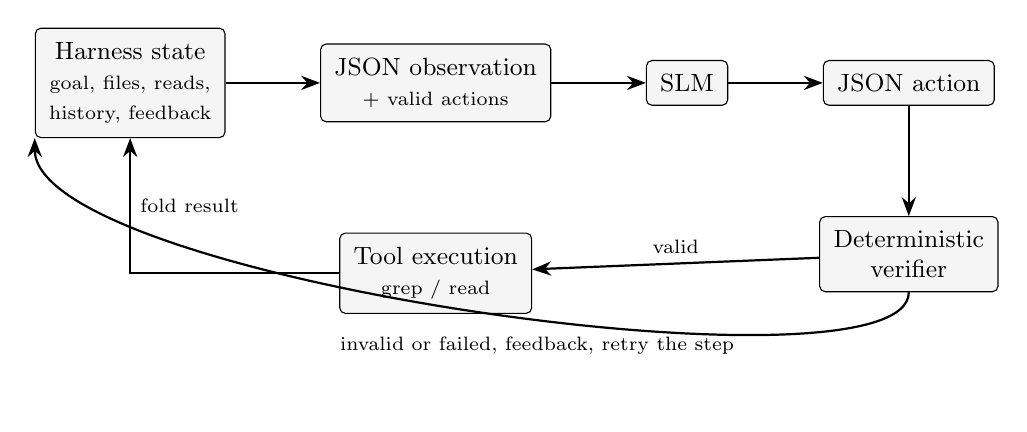
\begin{tikzpicture}[
      node distance=14mm and 12mm,
      box/.style={draw, rounded corners=2pt, align=center, inner sep=5pt,
                  font=\small, fill=gray!8},
      arr/.style={-{Stealth[length=2.4mm]}, thick}
    ]
    \node[box] (state)  {Harness state\\\scriptsize goal, files, reads,\\\scriptsize history, feedback};
    \node[box, right=of state] (obs)    {JSON observation\\\scriptsize + valid actions};
    \node[box, right=of obs]   (model)  {SLM};
    \node[box, right=of model] (action) {JSON action};
    \node[box, below=of action] (verify) {Deterministic\\verifier};
    \node[box, below=of obs] (tool) {Tool execution\\\scriptsize grep / read};
    \draw[arr] (state) -- (obs);
    \draw[arr] (obs) -- (model);
    \draw[arr] (model) -- (action);
    \draw[arr] (action) -- (verify);
    \draw[arr] (verify) -- node[above, font=\scriptsize]{valid} (tool);
    \draw[arr] (tool) -| node[near end, right, font=\scriptsize]{fold result} (state.south);
    \draw[arr] (verify.south) .. controls +(0,-14mm) and +(0,-18mm) .. (state.south west)
      node[pos=0.45, below=1mm, font=\scriptsize]{invalid or failed, feedback, retry the step};
  \end{tikzpicture}
  \caption{One step of the custom harness. The model is stateless between
  steps. Verification happens before an action counts, and a failed step is
  retried alone with the failure reason visible in the next observation.}
  \label{fig:loop}
\end{figure}

% ---------------------------------------------------------------- 5
\section{Distillation and training}

The training data problem for a narrow role is that no public dataset speaks
a bespoke harness schema. We manufacture the data. The 72B teacher runs every
training-split task inside both harnesses. Only trajectories that pass both
the per-step verifier and the final answer scorer are kept. Custom-harness
steps become observation-action pairs verbatim. Generic-harness trajectories
are replayed through the custom state machine so that each tool call is
re-expressed as a schema-valid action paired with the exact observation a
student would see at inference time.

In the published run the teacher attempted 320 trajectories and 303 came out
verifier-clean, which yielded 428 training examples with 48 for validation
and 57 held out. Each student is fine-tuned with LoRA \citep{hu2022lora} at
rank 64 and alpha 128 for three epochs, then merged to fp16 and served like
any base model with vLLM \citep{kwon2023vllm}. Training the 3B student took
under four minutes on the same GPU used for serving and cost about eighteen
cents at the quoted rate.

% ---------------------------------------------------------------- 6
\section{Experimental design}

\subsection{The factorial grid}

Table~\ref{tab:grid} shows the six conditions. The grid crosses three model
classes with two harnesses. C1 is the economically relevant baseline, namely
the large model in the standard interface. C5 is the proposed system. C6
probes whether the custom harness alone transfers to the large model.

\begin{table}[t]
  \centering
  \small
  \caption{The six experimental conditions.}
  \label{tab:grid}
  \begin{tabular}{lcc}
    \toprule
     & generic harness & custom harness \\
    \midrule
    large general model (72B) & \textbf{C1} baseline & \textbf{C6} harness transfer probe \\
    small general model       & \textbf{C2} naive cost cut & \textbf{C3} harness only \\
    small fine-tuned model    & \textbf{C4} fine-tuning only & \textbf{C5} proposed \\
    \bottomrule
  \end{tabular}
\end{table}

From the small-model two-by-two sub-grid we compute, on any metric, the
harness effect as $C3 - C2$, the fine-tuning effect as $C4 - C2$, an additive
prediction for C5 as $C3 + C4 - C2$ and the interaction as the observed C5
minus that prediction. A large positive interaction on success means the two
interventions amplify each other, which is the signature of genuine
co-design rather than stacked independent improvements.

\subsection{Models and hardware}

Every model is an open Qwen2.5 instruction-tuned checkpoint \citep{qwen25}.
The teacher and large-model conditions use Qwen2.5-72B-Instruct in the
official AWQ four-bit release \citep{lin2024awq}, which fits a single
94\,GB NVIDIA H100 NVL alongside its KV cache. Students are the 7B, 3B and
1.5B instruction-tuned checkpoints. Everything is served with vLLM 0.7.3
\citep{kwon2023vllm} on one card rented at \$3.19 per hour. One model is
resident at a time and all conditions run sequentially on the same card, so
costs are directly comparable.

\subsection{The cost model}

Cost is grounded in measured hardware throughput rather than a vendor price
list. For each served model we measure realized prefill and decode tokens per
second, then convert the GPU's hourly price into a per-token price. The 72B
teacher is therefore correctly costlier per token than the students. The
one-time fine-tuning cost is measured wall-clock training time at the same
hourly rate and enters the break-even analysis. Because every condition
shares one GPU at one rate, the headline ratios between conditions do not
depend on the rate chosen.

\subsection{Statistics}

Success per condition carries a Wilson 95 percent interval
\citep{wilson1927}. Success comparisons between conditions use the exact
two-sided McNemar test on paired per-task outcomes \citep{mcnemar1947},
which uses only the tasks where the two conditions disagree. Cost-ratio
uncertainty comes from a paired task-level percentile bootstrap with ten
thousand resamples \citep{efron1979}. All statistics are computed by a small
self-contained module in the repository and can be regenerated offline from
the committed run logs with one command.

% ---------------------------------------------------------------- 7
\section{Results}

\subsection{Main results}

Table~\ref{tab:main} reports the full grid for the 3B student, which is the
headline configuration. Figures~\ref{fig:success} and~\ref{fig:cost} plot
success and cost per successful task by condition.

\begin{table}[t]
  \centering
  \small
  \caption{Main results for the 3B grid. Two hundred held-out tasks per
  condition, one attempt per task at temperature zero. Intervals are Wilson
  95 percent.}
  \label{tab:main}
  \begin{tabular}{lccc}
    \toprule
    Condition & Success [95\% CI] & Cost per success & Cost per attempt \\
    \midrule
    C1 72B + generic (baseline) & 0.955 [0.917, 0.976] & \$0.010252 & \$0.009791 \\
    C2 3B + generic (naive swap) & 0.480 [0.412, 0.549] & \$0.013908 & \$0.006676 \\
    C3 3B + custom & 0.250 [0.195, 0.314] & \$0.010199 & \$0.002550 \\
    C4 3B-FT + generic & 0.410 [0.344, 0.479] & \$0.009759 & \$0.004001 \\
    \textbf{C5 3B-FT + custom (ours)} & \textbf{0.945 [0.904, 0.969]} & \textbf{\$0.001558} & \textbf{\$0.001472} \\
    C6 72B + custom & 0.810 [0.750, 0.858] & \$0.022736 & \$0.018417 \\
    \bottomrule
  \end{tabular}
\end{table}

\begin{figure}[t]
  \centering
  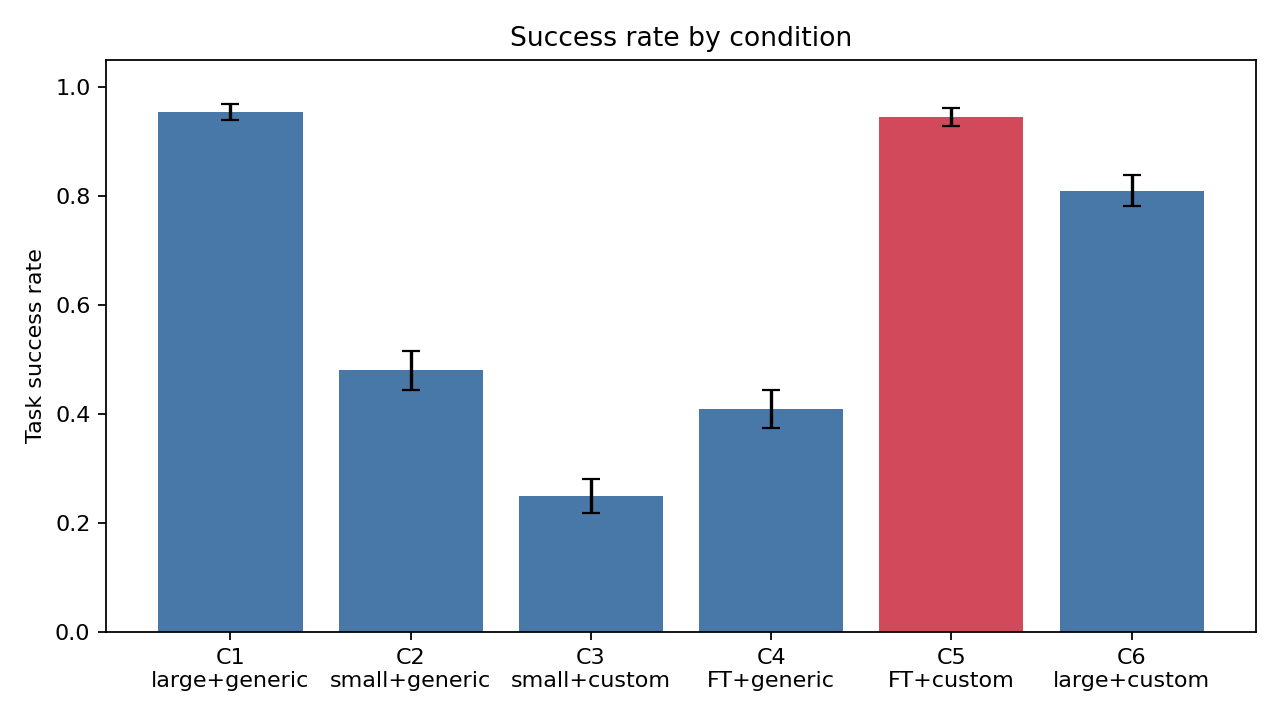
\includegraphics[width=0.78\textwidth]{figures/fig1_success_by_condition.png}
  \caption{Success rate by condition for the 3B grid.}
  \label{fig:success}
\end{figure}

\begin{figure}[t]
  \centering
  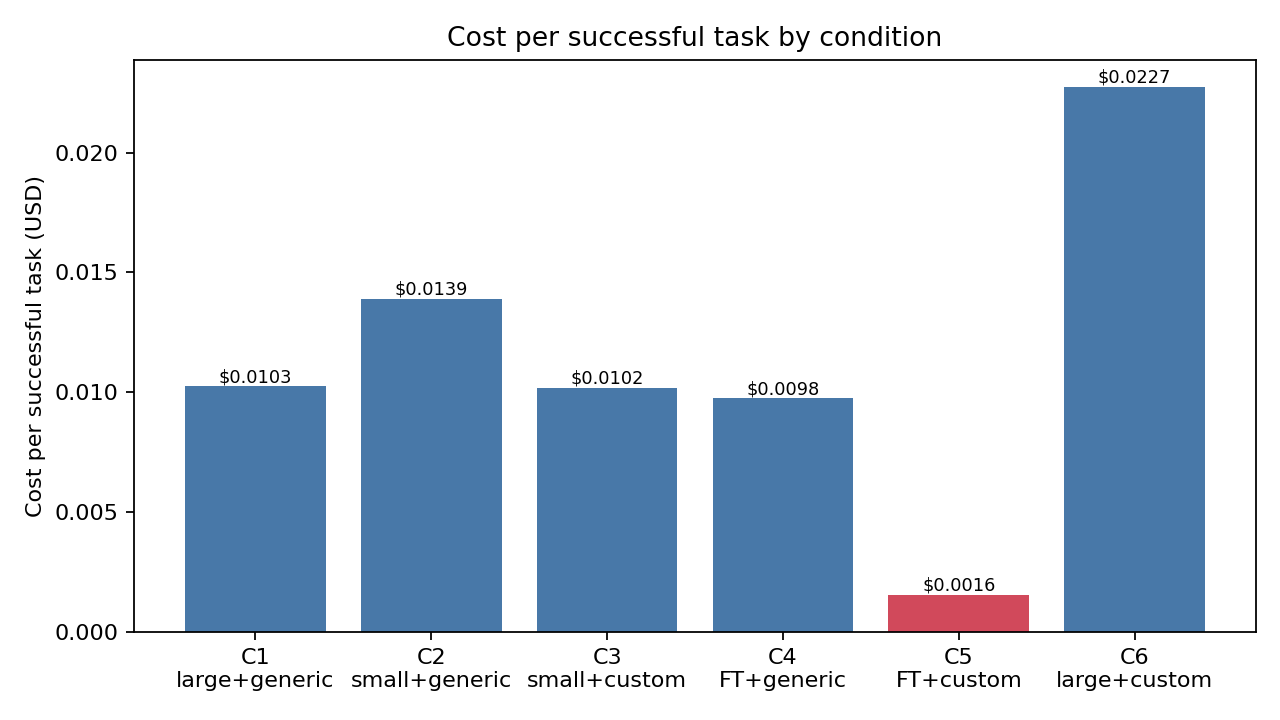
\includegraphics[width=0.78\textwidth]{figures/fig2_cost_per_success.png}
  \caption{Cost per successful task by condition for the 3B grid.}
  \label{fig:cost}
\end{figure}

\subsection{The primary claim}

We pre-registered the claim that the specialist cuts cost per successful task
by at least half while losing no more than two points of success. Against the
strong baseline the 3B specialist reduces cost per success by 84.8 percent
with a bootstrap 95 percent interval of [83.3, 86.1], so the entire interval
clears the target with room to spare. Success moves from 0.955 to 0.945. On
the 200 shared tasks the two systems disagree on twenty, with nine won only
by the specialist and eleven won only by the baseline, and the exact McNemar
test gives $p = 0.82$. The success rates are statistically
indistinguishable. The claim holds, and the specialist costs about one
seventh as much per completed task.

\subsection{The naive swap fails on both axes}

C2 is the move practitioners actually make, namely dropping the same small
model into the standard interface and hoping the price sheet wins. It does
not. Success collapses to 0.480 against 0.955, with ninety-eight tasks won
only by the baseline against three won only by C2 and $p = 1.4 \times
10^{-25}$. Cost per successful task rises above the baseline, with a ratio of
1.36 and a bootstrap interval of [1.04, 1.77] that excludes parity. Failure
amplifies spending. The 7B variant of the naive swap burns twice the input
tokens per attempt of the baseline on retries and corrections. Cheap tokens
do not make a cheap worker.

\subsection{Attribution and the co-design interaction}

\begin{figure}[t]
  \centering
  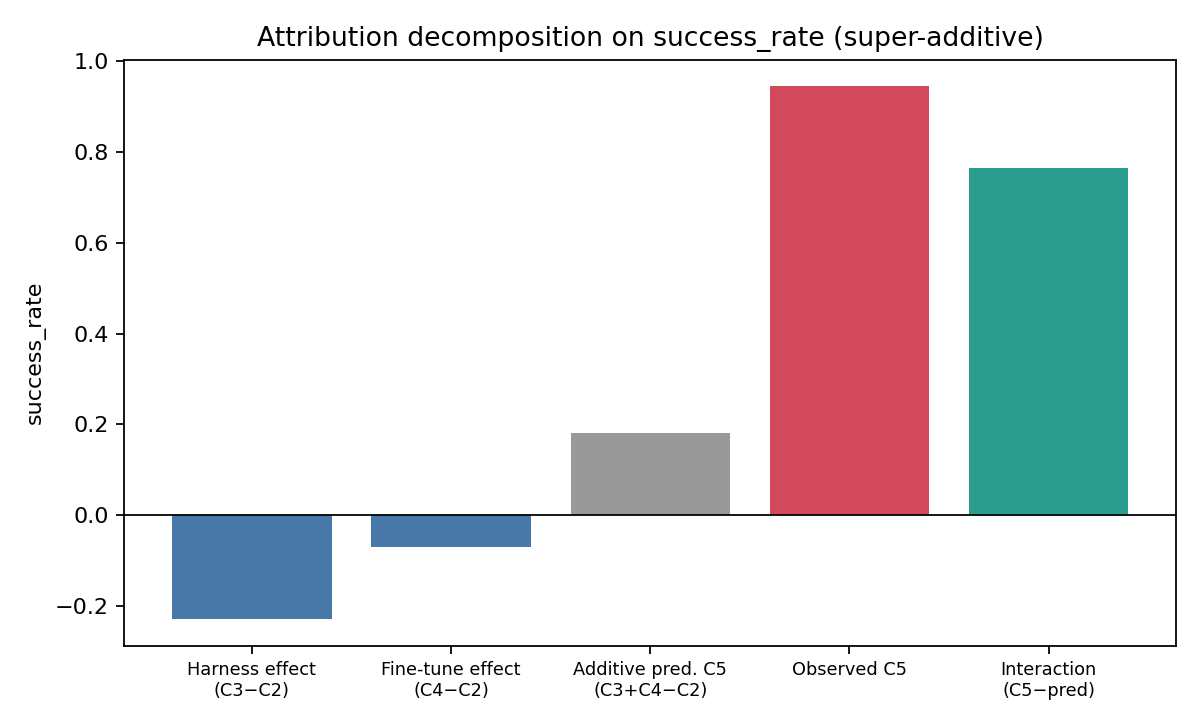
\includegraphics[width=0.78\textwidth]{figures/fig3_attribution_success.png}
  \caption{Attribution on success for the 3B grid. The interaction term
  dwarfs both individual effects, and both individual effects are negative.}
  \label{fig:attr}
\end{figure}

On the 3B grid the harness effect on success is $-0.230$ and the fine-tuning
effect is $-0.070$. The additive prediction for C5 is therefore 0.180. The
observed C5 is 0.945, which makes the interaction $+0.765$
(Figure~\ref{fig:attr}). Each ingredient alone made things worse and the
combination approached the 72B.

The mechanism is visible in the failure modes. The untrained 3B inside the
strict schema (C3) averaged 2.75 invalid actions per attempt. The 72B inside
the same schema (C6) still averaged 0.19 invalid actions per attempt and
landed at 0.810, well under its own generic-harness score, so the custom
interface is genuinely hard zero-shot rather than secretly easy. The
fine-tuned 3B inside the schema it was trained for (C5) averaged 0.03 invalid
actions per attempt. The sharpest version of the story is the 1.5B student.
Fine-tuned and placed in the \emph{generic} interface it scores 0.010.
The identical weights placed in the harness they were co-designed with score
0.935. The capability the fine-tune installs is only expressible inside the
interface it was designed against, which is what co-design means
operationally.

\subsection{Generalization across repositories}

\begin{table}[t]
  \centering
  \small
  \caption{Per-repository success of the baseline and the 3B specialist.
  Forty tasks per repository.}
  \label{tab:repos}
  \begin{tabular}{lcc}
    \toprule
    Test repository & C1 (72B + generic) & C5 (3B specialist) \\
    \midrule
    private corpus & 1.000 (40/40) & 0.950 (38/40) \\
    flask          & 1.000 (40/40) & 0.975 (39/40) \\
    click          & 0.950 (38/40) & 0.875 (35/40) \\
    rich           & 1.000 (40/40) & 0.975 (39/40) \\
    httpx          & 0.825 (33/40) & \textbf{0.950 (38/40)} \\
    \bottomrule
  \end{tabular}
\end{table}

Table~\ref{tab:repos} breaks the headline out by repository. The specialist
stays between 0.875 and 0.975 everywhere, including on four repositories it
never saw during distillation, and it beats the baseline outright on httpx,
which happens to be the baseline's weakest repository. The result is not an
artifact of one codebase.

\subsection{The size sweep}

\begin{table}[t]
  \centering
  \small
  \caption{The specialist (C5) against the same 72B baseline across student
  sizes. Discordant counts are tasks won only by the specialist against tasks
  won only by the baseline.}
  \label{tab:sweep}
  \begin{tabular}{lcccc}
    \toprule
    Student & Success [95\% CI] & Discordant, $p$ & Cost per success & Reduction [95\% CI] \\
    \midrule
    7B  & 0.920 [0.874, 0.950] & 8/15, $p=0.21$ & \$0.002441 & 76.2\% [74.2, 78.1] \\
    \textbf{3B} & \textbf{0.945 [0.904, 0.969]} & 9/11, $p=0.82$ & \textbf{\$0.001558} & \textbf{84.8\% [83.3, 86.1]} \\
    1.5B & 0.935 [0.892, 0.962] & 9/13, $p=0.52$ & \$0.001787 & 82.6\% [80.5, 84.3] \\
    \bottomrule
  \end{tabular}
\end{table}

Table~\ref{tab:sweep} repeats the comparison at three student sizes trained
on identical data with an identical recipe. Every size is statistically
indistinguishable from the baseline on success while cutting cost per
success by 76 to 85 percent. Only the 3B meets the strict two-point criterion
on the point estimate. The ordering is not monotonic in size, since the 7B
trails the 3B. With a fixed 428-example budget and three epochs the smaller
models appear to adopt the schema more completely while the 7B retains more
of its general-purpose habits. We report this as observed and leave per-size
tuning to future work. It is worth pausing on the 1.5B row. The harness
carries a model of that size to 0.935 even though the same fine-tuned weights
score 0.010 in the generic interface.

\subsection{Break-even}

\begin{figure}[t]
  \centering
  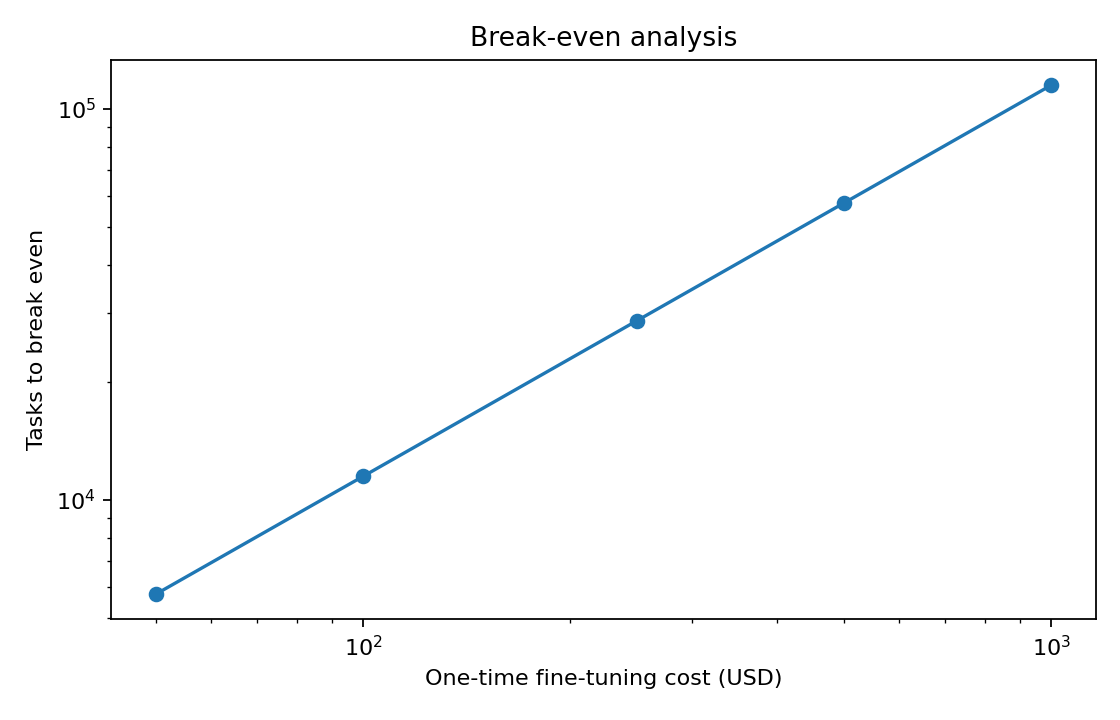
\includegraphics[width=0.7\textwidth]{figures/fig5_break_even.png}
  \caption{Cumulative cost against completed tasks. The one-time fine-tune
  pays for itself after roughly twenty-one successful tasks.}
  \label{fig:breakeven}
\end{figure}

Fine-tuning the 3B cost \$0.18 of measured GPU time. The specialist saves
\$0.0087 per successful task against the baseline, so the fine-tune pays for
itself after about twenty-one successful tasks (Figure~\ref{fig:breakeven}).
Any realistic deployment amortizes it to nothing.

\subsection{Replication at smaller scale}

An earlier complete run of the same pipeline used a 14B teacher on a 48\,GB
card with a single test repository of forty tasks. Its baseline was weaker at
0.725 and the 3B specialist beat it outright while cutting cost per success
by 74.9 percent with a bootstrap interval of [63.8, 84.0]. The direction of
the result survived a five-fold change in teacher scale and a five-fold
change in test-set size. Both runs' raw logs live in the repository history.

% ---------------------------------------------------------------- 8
\section{Engineering findings worth keeping}

Several failures along the way changed the results materially and are part of
the honest record. They are all fixed in the released code with regression
tests.

\begin{itemize}
  \item vLLM rejects OpenAI-style automatic tool choice unless launched with
        the right parser flags, and the failure mode silently zeroes the
        baseline rather than crashing. Every generic-harness condition
        depends on those two flags.
  \item The benchmark's split labels and the fine-tuning data's split labels
        are different concepts. Conflating them starved the validation file
        and aborted training.
  \item Models occasionally emit malformed glob patterns. The path libraries
        underneath the grep and glob tools raise on those patterns, and an
        uncaught raise killed entire evaluation processes mid-run on two
        occasions. Tool errors must be returned to the agent loop as
        feedback, never propagated.
  \item Temperature-zero decoding means nominal seeds replay identical
        trajectories. Treating replays as independent samples silently
        overstates precision by about $\sqrt{2}$. Our analysis deduplicates
        to one attempt per task and the released statistics module makes
        that the default.
  \item A harness rule the designer thinks is obvious is not obvious to the
        model. Until the prompt stated that answering requires a prior read,
        the teacher burned its retries re-emitting the same forbidden action.
        One sentence in the prompt moved teacher trajectory yield from 21
        clean trajectories out of 240 to 170 out of 240 in the smaller run.
\end{itemize}

% ---------------------------------------------------------------- 9
\section{Limitations}

\begin{itemize}
  \item One role and one task family so far. File navigation is high-volume
        and verifiable, which made it the right Phase 1 target, and a second
        role such as test execution with failure localization is the obvious
        next step.
  \item The baseline is an open 72B in a four-bit AWQ release. A frontier API
        model might score somewhat higher than 0.955, though the Wilson floor
        of 0.917 leaves limited headroom. A small frontier-API anchor slice
        would settle this cheaply.
  \item Five repositories and 200 tasks bound the precision of per-repository
        cells at forty tasks each. More repositories would tighten them.
  \item The 7B's underperformance relative to the 3B under an identical
        recipe is reported rather than explained. Per-size tuning was
        deliberately withheld for comparability.
  \item Absolute dollar figures scale with the GPU rate and the measured
        throughput. Ratios between conditions do not, because every condition
        shares one card at one rate.
\end{itemize}

% ---------------------------------------------------------------- 10
\section{Reproducibility}

The repository at \repo{} contains the harnesses, the verifier, the benchmark
generator, the distillation pipeline, the training and serving scripts, the
statistics module, every run log behind every number in this paper, the
fine-tuning data and the figure generation code. The offline checks need no
GPU. The full experiment is one script on one rented 80\,GB-class GPU and
finished in about ninety minutes for roughly five dollars. The statistics
reproduce from the frozen logs with a single command, and the test suite runs
in under two seconds on a laptop.

% ---------------------------------------------------------------- 11
\section{Conclusion}

We asked whether a fine-tuned small model inside a co-designed harness can
replace an expensive general worker without giving up reliability. Against a
strong 72B baseline succeeding 95.5 percent of the time, a 3B specialist
succeeded 94.5 percent of the time at one seventh of the cost per completed
task, the gap statistically indistinguishable, the result stable across five
held-out repositories and three student sizes and consistent with an
independent smaller-scale replication. The factorial decomposition shows why
naive approaches disappoint. The harness alone hurts. Fine-tuning alone
hurts. The pair, designed together, recovers nearly all of the large model's
reliability because the small model was taught to live inside exactly the
structure that keeps it safe. Specialized subagents, not merely smaller ones,
are the cost-efficient building block for multi-agent systems.

\bibliographystyle{plainnat}
\bibliography{refs}

\end{document}
